%---------------------------------------------------------------------------%
%->> Frontmatter
%---------------------------------------------------------------------------%
%-
%-> 生成封面
%-
\maketitle% 生成中文封面
\MAKETITLE% 生成英文封面
%-
%-> 作者声明
%-
\makedeclaration% 生成声明页
%-
%-> 中文摘要
%-
\intobmk\chapter*{摘\quad 要}% 显示在书签但不显示在目录
\setcounter{page}{1}% 开始页码
\pagenumbering{Roman}% 页码符号

目标跟踪是计算机视觉领域中最重要和最具挑战性的研究课题之一,在智能监控、自动驾驶等领域有着潜在广阔的应用前景。目标跟踪的核心是估计图像序列的每帧中目标的运动状态。目标跟踪是计算机视觉领域的中层部分,为目标的行为理解提供了基础,因此具有非常重要的理论研究价值。同时,它具有广泛的实际应用,包括视频监控,交通流量监控,视频压缩和人机交互等。
%例如,目标跟踪已成功应用于监控居民区,停车场和银行中的人类活动(例如W4系统[1]和VSAM项目[2])。在交通运输领域,目标跟踪也被广泛用于交通流量监控[3],行人计数[4]等任务。由于目标跟踪的理论价值与应用价值,众多科研机构和公司都投入到这项研究中。
然而,目标跟踪领域存在很多理论和技术问题有待解决,如运动模糊、光照变化、非刚性目标的形变、视角的变化导致的目标旋转、遮挡等。近年来深度学习的突破为解决目标跟踪中的一系列问题带来了可能。
深度学习是基于人工神经网络的机器学习方法。在过去的十年中,深度学习技术得到了飞速发展,已成功应用于计算机视觉,语音识别,自然语言处理,音频识别,社交网络过滤,机器翻译,生物信息学,药物设计等领域。如何利用深度学习方法,尤其是深度卷积神经网络解决跟踪过程中遇到的复杂问题,具有较大的研究价值和研究空间。

本文利用卷积神经网络强大的表征能力,为视频目标跟踪算法的特征表示,表观模型建模,运动模型建模,模型自适应等方面进行了改进,有效提高的算法的性能。同时,本文将对抗性信息应用到视频目标跟踪任务中,以研究视频目标跟踪算法相对于对抗样本的鲁棒性。本文的主要工作和贡献概括如下:

\begin{figure}
\centering
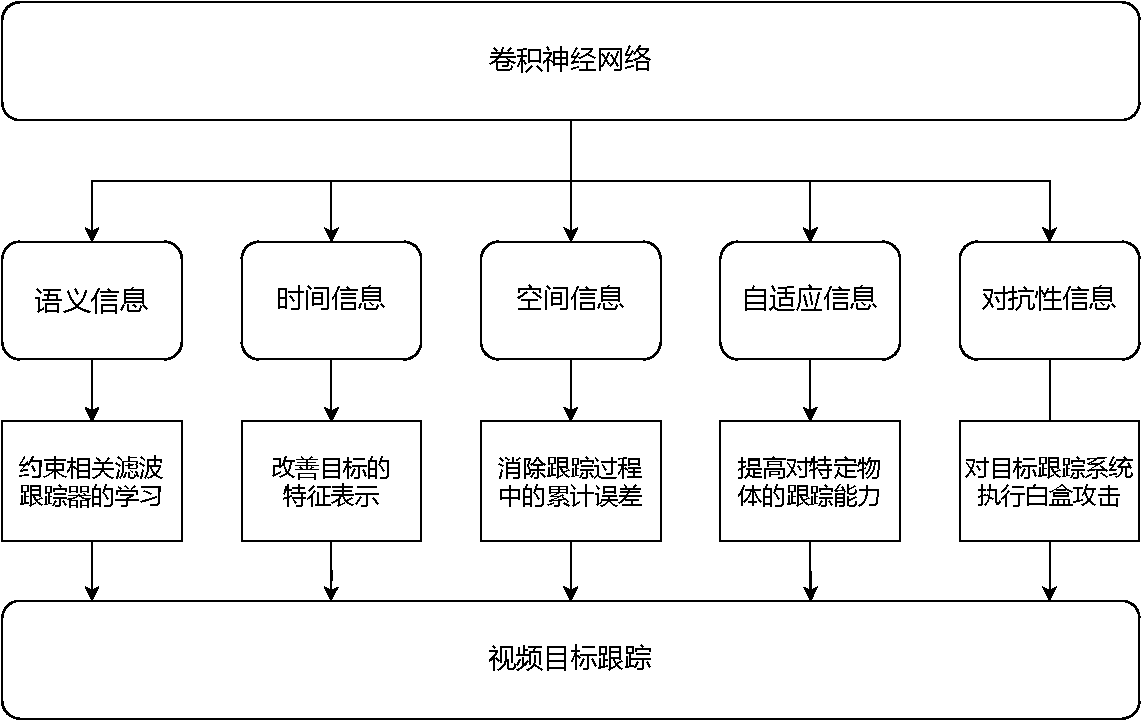
\includegraphics[width=0.75\textwidth]{Img/paper_arch.pdf}
\caption{文章组织架构}
\end{figure}

\begin{itemize}
\item{\textbf{提出了一种语义信息引导的视频目标跟踪算法。}该算法利用卷积神经网络获得目标的\textbf{语义信息},用于约束跟踪器的训练过程,从而提高跟踪的效果。具体而言:首先,我们提出了实例引导的相关滤波器,利用卷积神经网络学习图像的实例级别的语义分割模板,从而约束相关滤波器的学习。其次,针对离线训练的语义分割结果和在线学习的相关滤波结果具有互补性这一特点,我们提出了跟踪结果的自纠正机制,利用分割结果纠正相关滤波结果。我们在多个具有挑战性的视频目标跟踪数据库上验证了这些创新点在视频目标跟踪应用中的有效性。}
\item{\textbf{提出了一种空间信息增强的视频目标跟踪算法。}该算法主要在运动模型方面对基于孪生网络的视频目标跟踪算法进行优化。具体而言:我们为孪生跟踪网络引入了更丰富的\textbf{空间信息},即始终在整个图像平面内感知物体的位置信息,能够弥补传统的局部搜索机制中目标搜索范围有限的缺点,从而有效地减少累积误差并提高鲁棒性。为了进一步减轻近似物体的干扰,我们提出了一个端到端训练的轨迹预测模块,能够利用物体的历史轨迹信息和当前帧的表观信息,预测目标在当前帧的每个空间位置上出现的可能性。我们在多个视频跟踪标准评测库上验证了这些创新点的有效性,并大幅度提高了跟踪算法的准确性和鲁棒性。}
\item{\textbf{提出了一种时间信息增强的视频目标跟踪算法。}该算法主要在特征提取方面对基于孪生网络的视频目标跟踪算法进行优化。首先,我们从基于孪生网络的在线视频跟踪算法鲁棒性不足问题出发,将\textbf{时间信息}引入在线视频目标跟踪中。通过来自相邻帧的目标表观信息的聚合,使得目标表观特征更加丰富,弥补基于孪生网络的视频目标跟踪算法局限于从单帧提取目标表观,从而对目标表观表示能力不足的缺点,从而提高跟踪的效果,实现鲁棒的跟踪。在端到端时间聚合的基础上,我们通过引入对抗性 Dropout 模块,并通过在大规模数据集上端到端训练,使得孪生网络跟踪器在目标由于运动模糊等导致的表观不佳的情况下具有更好的表现,从而进一步提高跟踪的鲁棒性。我们在目前流行的视频目标跟踪评测库上进行了算法的对比试验以及成分分析实验,从而验证算法改进的有效性。}
\item{\textbf{提出了一种自适应信息增强的视频目标跟踪算法。}该算法主要在模型自适应方面对基于孪生网络的视频目标跟踪算法进行优化。我们为孪生跟踪网络引入了\textbf{自适应信息},通过对模板图像的像素进行微小的扰动,改善孪生网络跟踪器对于特定目标的跟踪性能。该自适应性信息通过对模板图像进行梯度的反向传播计算得到,能够以即插即用的方式轻松添加到现有孪生网络跟踪器中,而无需修改网络模型的参数。在线跟踪时,仅在第一帧进行数次梯度传播和模板图像像素值更新,即可实现目标的实时跟踪。我们同样在多个视频目标跟踪评测库上验证了算法的有效性,并在精确度与实时性上取得了较好的结果。}
\item{\textbf{将对抗性信息应用于基于孪生网络的视频目标跟踪算法。}该算法将\textbf{对抗性信息}应用到孪生跟踪网络中,以研究视频目标跟踪算法相对于对抗样本的鲁棒性。具体而言,我们为基于孪生网络的视频目标跟踪算法生成视频无关的通用扰动,从而使得跟踪器做出错误的行为。我们为模板图像添加微小的扰动,为搜索图像添加小的补丁,这样,跟踪器预测到补丁的位置而不是目标的位置。通过离线的大规模视频目标跟踪数据集训练对抗性扰动信息,从而实现有效的攻击。我们在多个视频目标跟踪标准评测库上验证了所提出的对抗性信息的有效性,同时验证了其在不同主干网络和不同跟踪框架的可迁移性。}
\end{itemize}

%基于上述方法和创新,我们的跟踪算法在多个公开数据集上都取得了当时最好或者领先的评测结果。同时,上述方法和创新,对于其他计算机视觉问题和应用,例如视频分割、视频姿态估计等,也有一定的借鉴意义。

\keywords{相关滤波,视频目标跟踪,深度学习,卷积神经网络}% 中文关键词
%-
%-> 英文摘要
%-
\intobmk\chapter*{Abstract}% 显示在书签但不显示在目录

Target tracking is one of the most important and challenging research topics in the field of computer vision, and it has potential and broad application prospects in the fields of intelligent surveillance and autonomous driving. The core of target tracking is to estimate the motion state of the target in each frame of the image sequence. Target tracking is the middle part of the computer vision field, which provides a basis for the understanding of target behavior, so it has very important theoretical research value. At the same time, it has a wide range of practical applications, including video surveillance, traffic flow monitoring, video compression, and human-computer interaction. For example, target tracking has been successfully applied to monitor human activities in residential areas, parking lots and banks (such as the W4 system [1] and the VSAM project [2]). In the field of transportation, target tracking is also widely used in traffic flow monitoring [3], pedestrian counting [4] and other tasks.
Due to the theoretical value and application value of target tracking, many scientific research institutions and companies have invested in this research. However, there are many theoretical and technical problems to be solved in the field of target tracking, such as motion blur, illumination changes, deformation of non-rigid targets, target rotation and occlusion caused by changes in viewing angle. In recent years, the breakthrough of deep learning has brought the possibility to solve a series of problems in target tracking.
Deep learning is a machine learning method based on artificial neural networks. In the past ten years, deep learning technology has been rapidly developed and has been successfully applied in computer vision, speech recognition, natural language processing, audio recognition, social network filtering, machine translation, bioinformatics, drug design and other fields. How to use deep learning methods, especially deep convolutional neural networks to solve the complex problems encountered in the tracking process, has great research value and research space.

This paper uses the powerful representation ability of convolutional neural network to improve the feature representation of video target tracking algorithm, appearance model modeling, motion model modeling, model update, etc., and effectively improve the performance of the algorithm. The main work and contributions are:

\begin{itemize}
\item{\textbf{ proposed a semantic information guided video target tracking algorithm. }We use the convolutional neural network to obtain the target \textbf{semantic information} to constrain the training process of the tracker, thereby improving the tracking effect. Specifically, first: We propose an example-guided correlation filter. Use the neural network to learn the instance-level semantic segmentation template of the image to constrain the learning of related filters. Secondly, in view of the complementarity between the semantic segmentation results of offline training and the correlation filtering results of online learning, we propose a self-correction mechanism for tracking results, using the segmentation results to correct the correlation filtering results. We have verified the effectiveness of these innovations in video target tracking applications on multiple challenging video target tracking databases. }
\item{\textbf{ proposed a video target tracking algorithm with enhanced spatial information. }Different from previous work, where the spatial search is done locally to determine the target location, we have introduced richer \textbf{spatial information}. Specifically, the tracking algorithm is optimized in terms of the motion model, and always perceives the position information of the object in the entire image plane, making up for the shortcomings of the limited target search range in the traditional local search mechanism, thereby effectively reducing the accumulated error and improving the robustness. Awesome. In order to further reduce the interference of similar objects, we propose an end-to-end training trajectory prediction module that can use the historical trajectory information of the object and the apparent information of the current frame to predict the possibility of the object appearing in each spatial position of the current frame . We verified the effectiveness of these innovations on multiple video tracking standard evaluation libraries, and greatly improved the accuracy and robustness of the tracking algorithm. }
\item{\textbf{ proposed a video target tracking algorithm enhanced by time information. } The algorithm mainly optimizes the video target tracking algorithm based on the twin network in feature extraction. First, we start from the problem of insufficient robustness of the online video tracking algorithm based on the twin network, and introduce \textbf{time information} into online video target tracking. Through the aggregation of the target appearance information from adjacent frames, the target appearance feature is enriched, and the video target tracking algorithm based on the twin network is limited to extracting the target appearance from a single frame, and thus the lack of ability to express the target appearance , Thereby improving the tracking effect and achieving robust tracking. On the basis of end-to-end time aggregation, we introduced an adversarial dropout module, and through end-to-end training on large-scale data sets, the Siamese network tracker can be used in situations where the target's appearance is not good due to motion blur, etc. Has better performance, thereby further improving the robustness of tracking. We have conducted algorithm comparison experiments and component analysis experiments on the currently popular video target tracking evaluation library to verify the effectiveness of the algorithm improvement. }
\item{\textbf{Propose an adaptive information-enhanced video target tracking algorithm} This algorithm mainly optimizes the video target tracking algorithm based on the twin network in the aspect of model adaptation. We introduced \textbf{adaptive information}. Previous work: offline training. Purpose: Improve the adaptive ability of the algorithm to specific objects. First, by slightly disturbing the pixels of the template image, the tracking performance of the twin network tracker for specific targets is improved. The adaptive information is obtained by back-propagating the gradient of the template image, and can be easily added to the existing twin network tracker in a pluggable manner without modifying the parameters of the network model. In online tracking, only a few times of gradient propagation and template image pixel value update are performed in the first frame to realize the fact tracking of the target. We also verified the effectiveness of the algorithm on multiple video target tracking evaluation libraries, and achieved good results in accuracy and real-time performance. }
\item{\textbf{Applying adversarial information to a video target tracking algorithm based on the Siamese network} We introduced \textbf{adversarial information} and proposed an adversarial attack algorithm. The purpose: to prove the robustness of the existing tracker Sex is not good. Specifically, we generate video-independent general disturbances for the video target tracking algorithm based on the twin network, which makes the tracker behave incorrectly. We add a small perturbation to the template image and a small patch to the search image so that the tracker predicts the location of the patch instead of the location of the target. Through the offline large-scale video target tracking data set training adversarial disturbance information, so as to achieve effective attacks. We verified the effectiveness of the proposed adversarial information on multiple video target tracking standard evaluation libraries, and at the same time verified its transferability in different backbone networks and different tracking frameworks. }
\end{itemize}

\KEYWORDS{Correlation Filter, Visual Object Tracking, Deep Learning, Conlvolutional Neural Network}% 英文关键词
%---------------------------------------------------------------------------%
